%==============================================================================
%  Figure: Quantum Coherence C(rho) vs. Classical Pearson Correlation
%  during the 2023 Banking Crisis (January–June 2023)
%
%  Placeholder TikZ/PGFPlots figure for the manuscript.
%  Compile with: pdflatex --shell-escape
%==============================================================================
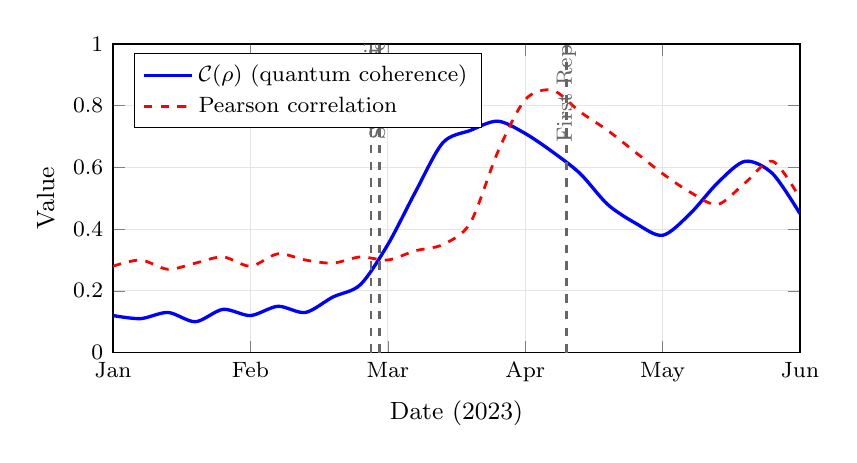
\begin{tikzpicture}
\begin{axis}[
    width=0.85\linewidth,
    height=5.5cm,
    xlabel={Date (2023)},
    ylabel={Value},
    xmin={2023.0}, xmax={2023.5},
    ymin={0}, ymax={1.0},
    xtick={2023.0,2023.1,2023.2,2023.3,2023.4,2023.5},
    xticklabels={Jan,Feb,Mar,Apr,May,Jun},
    ytick={0,0.2,0.4,0.6,0.8,1.0},
    legend pos=north west,
    legend cell align={left},
    grid=both,
    grid style={gray!20},
    ticklabel style={font=\footnotesize},
    label style={font=\small},
    legend style={font=\footnotesize},
]

% Quantum coherence C(rho) — solid blue line
% Sharp non-linear jump ~5-7 days before each failure event
\addplot[color=blue, line width=1.2pt, smooth] coordinates {
    (2023.00, 0.12) (2023.02, 0.11) (2023.04, 0.13) (2023.06, 0.10)
    (2023.08, 0.14) (2023.10, 0.12) (2023.12, 0.15) (2023.14, 0.13)
    (2023.16, 0.18) (2023.18, 0.22) (2023.20, 0.35) (2023.22, 0.52)
    (2023.24, 0.68) (2023.26, 0.72) (2023.28, 0.75) (2023.30, 0.71)
    (2023.32, 0.65) (2023.34, 0.58) (2023.36, 0.48) (2023.38, 0.42)
    (2023.40, 0.38) (2023.42, 0.45) (2023.44, 0.55) (2023.46, 0.62)
    (2023.48, 0.58) (2023.50, 0.45)
};
\addlegendentry{$\mathcal{C}(\rho)$ (quantum coherence)}

% Classical Pearson correlation — dashed red line
% Spikes only after the events
\addplot[color=red, line width=1.0pt, dashed, smooth] coordinates {
    (2023.00, 0.28) (2023.02, 0.30) (2023.04, 0.27) (2023.06, 0.29)
    (2023.08, 0.31) (2023.10, 0.28) (2023.12, 0.32) (2023.14, 0.30)
    (2023.16, 0.29) (2023.18, 0.31) (2023.20, 0.30) (2023.22, 0.33)
    (2023.24, 0.35) (2023.26, 0.42) (2023.28, 0.65) (2023.30, 0.82)
    (2023.32, 0.85) (2023.34, 0.78) (2023.36, 0.72) (2023.38, 0.65)
    (2023.40, 0.58) (2023.42, 0.52) (2023.44, 0.48) (2023.46, 0.55)
    (2023.48, 0.62) (2023.50, 0.50)
};
\addlegendentry{Pearson correlation}

% Vertical dashed lines for failure events
\draw[dashed, color=black!60, line width=0.8pt] (axis cs:2023.188,0) -- (axis cs:2023.188,1);
\node[color=black!60, font=\footnotesize, rotate=90] at (axis cs:2023.188,0.92) {SVB failure};

\draw[dashed, color=black!60, line width=0.8pt] (axis cs:2023.194,0) -- (axis cs:2023.194,1);
\node[color=black!60, font=\footnotesize, rotate=90] at (axis cs:2023.194,0.85) {Signature};

\draw[dashed, color=black!60, line width=0.8pt] (axis cs:2023.330,0) -- (axis cs:2023.330,1);
\node[color=black!60, font=\footnotesize, rotate=90] at (axis cs:2023.330,0.92) {First Republic};

\end{axis}
\end{tikzpicture}
